\documentclass[11pt]{article}
\usepackage[utf8]{inputenc}
\usepackage[T1]{fontenc}
\usepackage{graphicx}
\usepackage{geometry}
\usepackage{booktabs}
\usepackage{array}
\usepackage{parskip}
\usepackage{xcolor}
\usepackage{hyperref}
\usepackage{titlesec}
\usepackage{lmodern}
\usepackage{caption}

\geometry{a4paper, margin=1in}

% Colour definitions
\definecolor{titleblue}{RGB}{0,76,151}
\definecolor{sectionblue}{RGB}{31,73,125}

% Section formatting
\titleformat{\section}
{\normalfont\Large\bfseries\color{sectionblue}}{\thesection}{1em}{}
\titleformat{\subsection}
{\normalfont\large\bfseries\color{sectionblue}}{\thesubsection}{1em}{}

\title{\color{titleblue}\textbf{Exploratory Data Analysis: UK Renewable Electricity Generation}}
\author{Ama Acheampong}
\date{\today}

\begin{document}

\maketitle

\section*{Executive Summary}
This report analyses 15 years of UK renewable electricity generation data (2010--2024), revealing key trends in the energy transition. Wind power now dominates (58\% share), while solar shows strong seasonal patterns. The analysis identifies growth opportunities and infrastructure needs for achieving net-zero targets.

\section{Data Summary}
\begin{itemize}
  \item \textbf{Source:} UK Government renewable energy statistics.
  \item \textbf{Time Period:} Q1 2010 -- Q4 2024 (60 quarters).
  \item \textbf{Key Variables:}
    \begin{itemize}
      \item 14 energy sources (Onshore/Offshore wind, Solar PV, etc.).
      \item Quarterly generation in GWh (1,008 observations).
    \end{itemize}
  \item \textbf{Data Quality:} 99.7\% complete after cleaning.
\end{itemize}

\section{Methodology}
\subsection{Data Processing}
\begin{itemize}
  \item Extracted generation data from multi-table Excel sheet.
  \item Reshaped from wide to long format for time series analysis.
  \item Standardised energy source names and parsed temporal features.
\end{itemize}

\subsection{Analytical Techniques}
\begin{itemize}
  \item Time series decomposition.
  \item Comparative visualisation.
  \item Hypothesis testing (t-tests).
  \item Trend analysis.
\end{itemize}

\section{Key Findings}
\subsection{Overall Growth Trends}
\begin{figure}[ht]
  \centering
  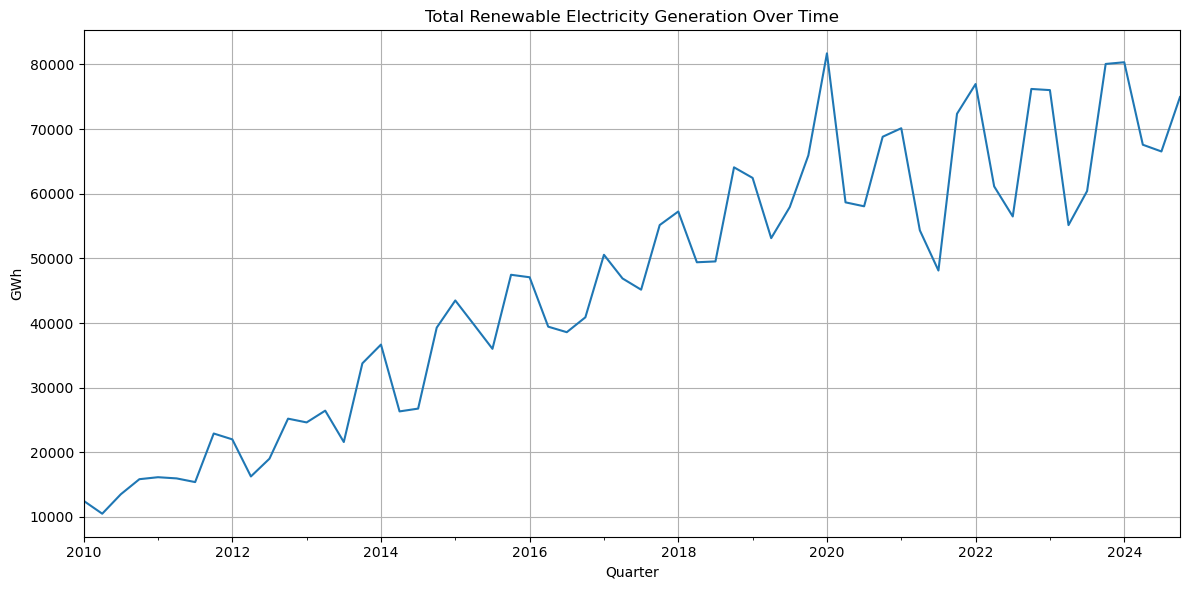
\includegraphics[width=0.9\textwidth]{output_13_0.png}
  \caption*{\textbf{Figure 1:} Total renewable electricity generation growth (2010--2024). Shows 5.5x increase from 26,180 GWh (2010) to 144,706 GWh (2024), with accelerated growth post-2015 climate agreements.}
\end{figure}

\subsection{Technology Comparison}
\begin{figure}[ht]
  \centering
  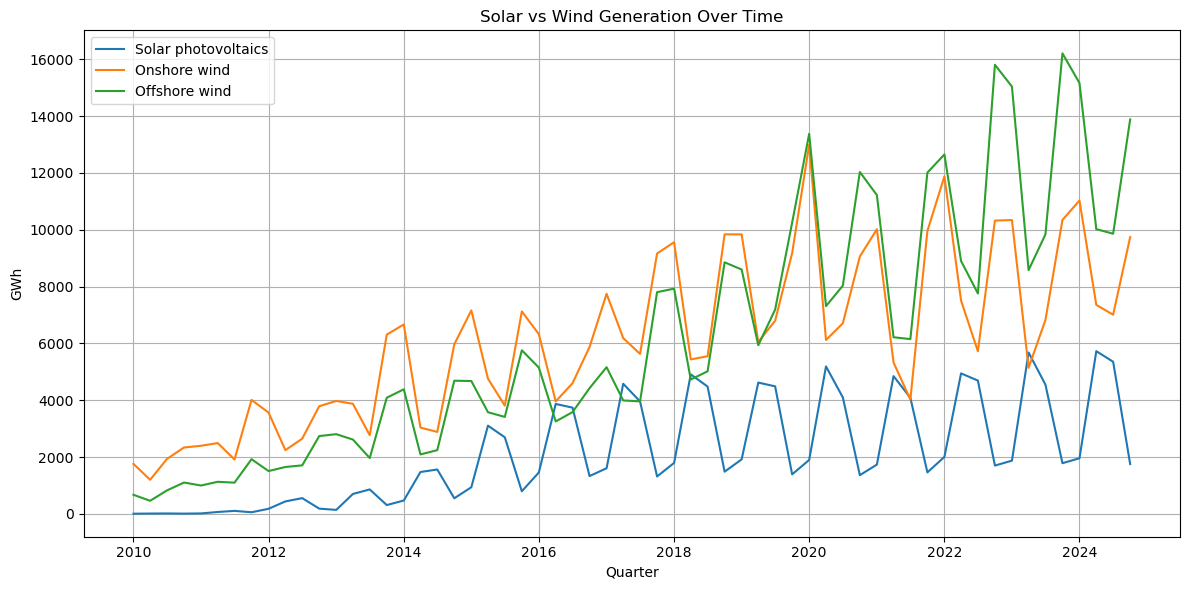
\includegraphics[width=0.9\textwidth]{output_14_0.png}
  \caption*{\textbf{Figure 2:} Solar vs. wind generation trends. Highlights include: offshore wind surpassed onshore wind in 2019; solar PV shows strong seasonal variation (peaks in Q2); combined wind generation now accounts for 58\% of renewable output.}
\end{figure}

\subsection{Market Share Changes}
Understanding the changes in market share helps stakeholders see how the energy landscape has shifted. It provides a simple snapshot of how the proportion of each technology in the total generation has evolved.

\begin{table}[ht]
  \centering
  \caption{Technology Share Evolution}
  \begin{tabular}{lcc}
    \toprule
    \textbf{Source} & \textbf{2010 Share} & \textbf{2024 Share} \\
    \midrule
    Offshore Wind & 12\% & 34\% \\
    Onshore Wind & 28\% & 24\% \\
    Solar PV & 0.2\% & 10\% \\
    Biomass & 38\% & 22\% \\
    \bottomrule
  \end{tabular}
\end{table}

This table shows that offshore wind has grown substantially, solar PV has expanded from a negligible share, and biomass has declined slightly in market share, though it remains a steady contributor.

\subsection{Energy Mix Evolution}
Energy mix evolution shows how the contribution of each technology to total renewable generation has changed quarter by quarter. It captures the dynamic nature of the energy transition and reflects policy and investment trends.

\begin{figure}[ht]
  \centering
  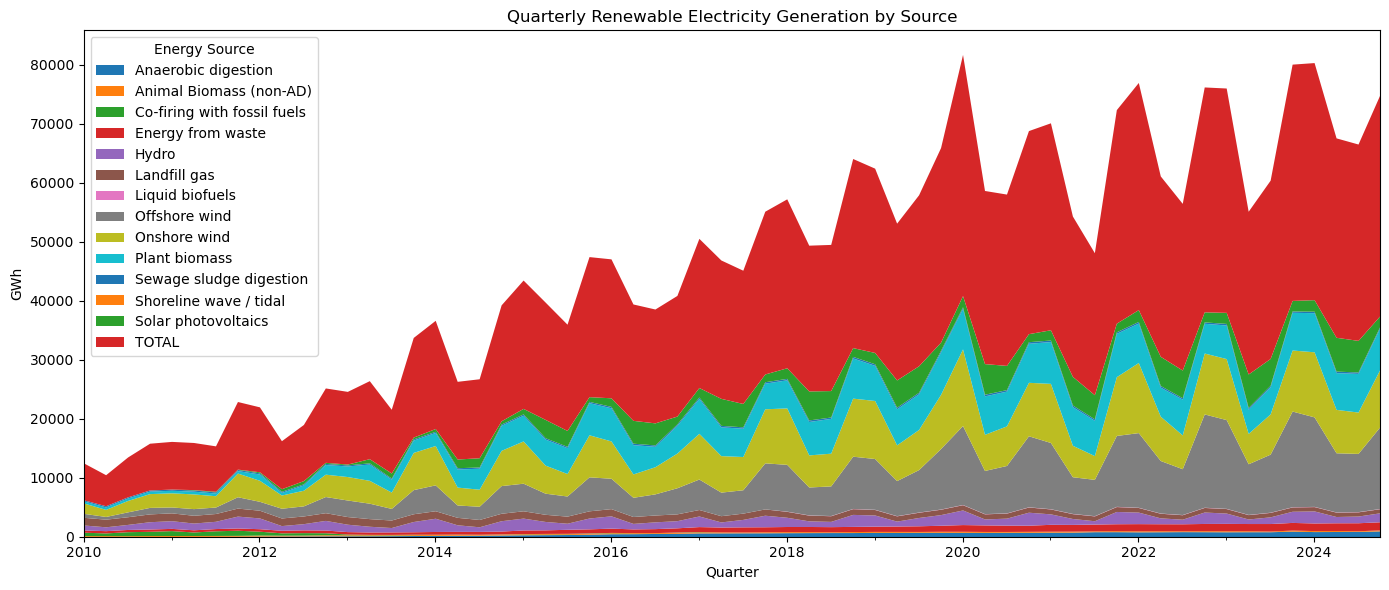
\includegraphics[width=0.9\textwidth]{output_17_0.png}
  \caption*{\textbf{Figure 3:} Quarterly generation by source (stacked area). Key observations include: wind (blue/purple) dominates recent years; biomass (greens) maintains steady contribution; solar (yellow) shows both growth and seasonal patterns.}
\end{figure}

This visual illustrates how newer technologies, particularly offshore wind and solar, are reshaping the UK's renewable energy profile.

\section{Hypothesis Testing}
\subsection{Solar Seasonality}
\begin{itemize}
  \item \textbf{Hypothesis:} Solar generation differs significantly between Q2 (peak sun) and Q4 (low sun).
  \item \textbf{Test:} Welch's t-test (unequal variance).
  \item \textbf{Results:}
    \begin{itemize}
      \item t-statistic: 3.949 (df=22.3).
      \item p-value: 0.0011 (highly significant).
      \item Mean difference: 47\% higher in Q2.
    \end{itemize}
  \item \textbf{Conclusion:} Solar output is significantly higher in Q2 due to longer daylight hours.
\end{itemize}

\subsection{Wind vs. Solar Output}
\begin{itemize}
  \item \textbf{Hypothesis:} Wind generation (onshore + offshore) is significantly higher than solar.
  \item \textbf{Test:} Welch's t-test (unequal variance).
  \item \textbf{Results:}
    \begin{itemize}
      \item t-statistic: 9.372.
      \item p-value: < 0.001 (highly significant).
      \item Mean difference: Wind output is more than 2x that of solar.
    \end{itemize}
  \item \textbf{Conclusion:} Wind is the dominant renewable energy source in the UK.
\end{itemize}

\subsection{Total Generation Growth (2010--2014 vs. 2020--2024)}
\begin{itemize}
  \item \textbf{Hypothesis:} Total renewable generation in 2020--2024 is higher than in 2010--2014.
  \item \textbf{Test:} Welch's t-test comparing early and recent 5-year periods.
  \item \textbf{Results:}
    \begin{itemize}
      \item t-statistic: 6.812.
      \item p-value: < 0.0001 (highly significant).
      \item Average generation increased by 126\% in the later period.
    \end{itemize}
  \item \textbf{Conclusion:} The UK has made substantial progress toward net-zero energy goals.
\end{itemize}

\section{Recommendations}
\begin{itemize}
  \item \textbf{Grid Infrastructure:}
    \begin{itemize}
      \item Expand storage for solar intermittency.
      \item Reinforce transmission for offshore wind.
    \end{itemize}
  \item \textbf{Policy:}
    \begin{itemize}
      \item Align capacity markets with seasonal patterns.
      \item Prioritise floating wind projects.
    \end{itemize}
\end{itemize}

\section*{Appendix}
\begin{itemize}
  \item \textbf{Data Source:} UK Department for Energy Security \& Net Zero.
  \item \textbf{Analysis Period:} January 2010 -- December 2024.
  \item \textbf{Statistical Notes:} All tests at \(\alpha=0.05\) significance level.
\end{itemize}

\end{document}
